\documentclass[11pt,a4paper]{article}
\usepackage[utf8]{inputenc}
\usepackage[T1]{fontenc}
\IfFileExists{lmodern.sty}{\usepackage{lmodern}}{}
\IfFileExists{french.ldf}{\usepackage[french]{babel}}{\usepackage[english]{babel}}
\usepackage{amsmath,amssymb,amsfonts,amsthm}
\usepackage{geometry}
\geometry{top=2cm, bottom=2cm, left=2.2cm, right=2.2cm}
\usepackage{booktabs,array,multirow}
\usepackage{enumitem}
\usepackage{xcolor}
\usepackage{tcolorbox}
\tcbuselibrary{skins,breakable}
\usepackage{tikz}
\usetikzlibrary{arrows.meta,positioning,shapes.geometric,calc}
\usepackage[colorlinks=true,linkcolor=blue!60!black]{hyperref}
\newtcolorbox{propbox}[1]{colback=blue!5!white,colframe=blue!75!black,fonttitle=\bfseries,title={#1},breakable,boxrule=0.8pt}
\newtcolorbox{rembox}[1]{colback=orange!5!white,colframe=orange!80!black,fonttitle=\bfseries,title={#1},breakable,boxrule=0.8pt}
\newtcolorbox{verifbox}{colback=green!4!white,colframe=green!45!black,fonttitle=\bfseries,title=Vérification algorithmique (Python),breakable,boxrule=0.6pt}
\newcommand{\Xt}{\tilde{X}}
\newcommand{\Yt}{\tilde{Y}}
\setlength{\parindent}{0pt}
\setlength{\parskip}{4pt}
\title{\textbf{Université Akli Mohand Oulhadj -- Bouira}\\
\large Master Recherche Opérationnelle (RO) -- 2025/2026\\
\Large \textbf{Théorie des Jeux : Solution Détaillée du TD n$^\circ$1}\\
\large Jeux matriciels à somme nulle}
\author{\textbf{Référence de cours :} Chapitre 1 (jeux matriciels)\\ Chapitre 2 (jeux antagonistes infinis)}
\date{}

\begin{document}
\maketitle
\hrule
\vspace{0.4cm}

\textbf{Conventions.} Le joueur 1 choisit les lignes et \emph{maximise} $a_{ij}$ ; le joueur 2 choisit les colonnes et \emph{minimise} $a_{ij}$ (sa perte). On note $L_i$ la ligne $i$, $C_j$ la colonne $j$, $\alpha=\max_i\min_j a_{ij}$ (valeur inférieure), $\beta=\min_j\max_i a_{ij}$ (valeur supérieure).

%=====================================================================
\section*{Exercice 1 : Stratégie dominée du joueur 2}

\[
A=\begin{pmatrix} 1 & 3 & 0\\ 1 & 2 & 4\end{pmatrix}, \qquad C_1=\begin{pmatrix}1\\1\end{pmatrix},\; C_2=\begin{pmatrix}3\\2\end{pmatrix},\; C_3=\begin{pmatrix}0\\4\end{pmatrix}.
\]

\begin{propbox}{Rappel du cours (pages 18, 22)}
Le joueur 2 minimise. La colonne $j^*$ est \textbf{dominée} par la colonne $\bar{j}$ si $a_{ij^*}\ge a_{i\bar{j}}$ pour tout $i$, avec au moins une inégalité stricte (\textbf{strictement dominée} si toutes les inégalités sont strictes). Dans l'extension mixte, $j_0$ est dominée s'il existe une stratégie mixte $q$ avec $q_{j_0}=0$ telle que $C_{j_0}\ge \sum_j q_j C_j$ (strictement si l'inégalité est stricte).
\end{propbox}

\paragraph{Comparaison $C_2$ / $C_1$.}
\[
a_{12}=3>1=a_{11},\qquad a_{22}=2>1=a_{21}.
\]
Toutes les inégalités sont strictes : $C_2$ est \textbf{strictement dominée} par $C_1$. Une stratégie pure étant une stratégie mixte particulière ($q=(1,0,0)$), $C_2$ est a fortiori strictement dominée dans l'extension mixte.

\paragraph{$C_3$ est-elle dominée ?} Il faudrait $q=(\mu,1-\mu,0)$ avec $\mu C_1+(1-\mu)C_2\le C_3$. Sur la ligne 1 : $\mu+3(1-\mu)=3-2\mu\ge 1>0=a_{13}$ pour tout $\mu\in[0,1]$. Impossible : \textbf{$C_3$ n'est pas dominée}.

\paragraph{$C_1$ est-elle dominée ?} Par $C_2$ : non ($C_2>C_1$). Par $C_3$ : non ($a_{23}=4>1$ mais $a_{13}=0<1$, il faudrait $C_1\ge C_3$). Par un mélange $\lambda C_2+(1-\lambda)C_3$ : ligne 2, $2\lambda+4(1-\lambda)=4-2\lambda\ge 2>1$, impossible. \textbf{$C_1$ n'est pas dominée.}

\[
\boxed{\begin{array}{c}\text{Oui : la stratégie 2 du joueur 2 est strictement dominée par sa stratégie 1}\\ \text{(donc aussi dans l'extension mixte).}\end{array}}
\]

\begin{rembox}{Prolongement : résolution complète}
Après suppression de $C_2$ : $\begin{pmatrix}1&0\\1&4\end{pmatrix}$. La ligne 2 domine la ligne 1 ($1\ge1$, $4>0$). Il reste $(1\;\;4)$ et le joueur 2 choisit $C_1$. Vérification directe sur $A$ : minima des lignes $0,1\Rightarrow\alpha=1$ ; maxima des colonnes $1,3,4\Rightarrow\beta=1$. Donc $\alpha=\beta=1=a_{21}$ : \textbf{point selle $(2,1)$, $v=1$}. (L'élément $a_{21}=1$ est minimal dans sa ligne et maximal dans sa colonne.)
\end{rembox}

%=====================================================================
\section*{Exercice 2 : Résolution graphique d'un jeu $2\times 3$}

\[
A=\begin{pmatrix} 2 & 6 & 0\\ 4 & 2 & 8\end{pmatrix}.
\]

\subsection*{1. Solution en stratégies pures ?}
\begin{align*}
\text{Minima des lignes : } & \min\{2,6,0\}=0,\quad \min\{4,2,8\}=2 \;\Rightarrow\; \alpha=\max\{0,2\}=2,\\
\text{Maxima des colonnes : } & \max\{2,4\}=4,\quad \max\{6,2\}=6,\quad \max\{0,8\}=8 \;\Rightarrow\; \beta=\min\{4,6,8\}=4.
\end{align*}
$\alpha=2<4=\beta$ : \boxed{\text{pas de point selle, donc pas de solution en stratégies pures.}}

\subsection*{2. Extension mixte}
\[
\Xt=\{x=(x_1,x_2)\in\mathbb{R}^2 : x_i\ge0,\ x_1+x_2=1\},\qquad \Yt=\{y=(y_1,y_2,y_3)\in\mathbb{R}^3 : y_j\ge0,\ y_1+y_2+y_3=1\},
\]
\[
E(x,y)=x^TAy=2x_1y_1+6x_1y_2+0\,x_1y_3+4x_2y_1+2x_2y_2+8x_2y_3,
\]
et l'extension mixte est $\tilde J=\langle I=\{1,2\},\Xt,\Yt,E\rangle$ ; le joueur 1 maximise $E$, le joueur 2 la minimise.

\subsection*{3. Gain minimal garanti du joueur 1 et stratégie optimale}
Posons $x=(p,1-p)$, $p\in[0,1]$. Le gain du joueur 1 contre chaque colonne pure est
\[
E(x,C_1)=2p+4(1-p)=4-2p,\qquad E(x,C_2)=6p+2(1-p)=2+4p,\qquad E(x,C_3)=8(1-p)=8-8p.
\]
Comme $E(x,\cdot)$ est linéaire en $y$, le minimum sur $\Yt$ est atteint en une colonne pure :
\[
\varphi(p)=\min_{y\in\Yt}E(x,y)=\min\{4-2p,\;2+4p,\;8-8p\}.
\]
\begin{center}
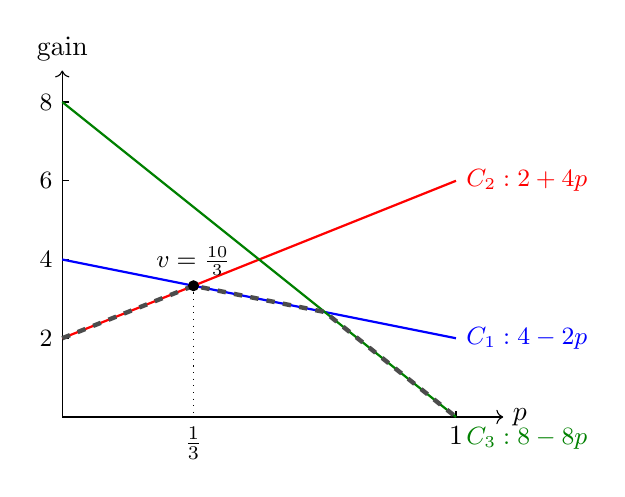
\begin{tikzpicture}[scale=1.0]
\draw[->] (0,0)--(5.6,0) node[right]{$p$};
\draw[->] (0,0)--(0,4.4) node[above]{gain};
\foreach \y in {2,4,6,8} \draw (0,\y/2) node[left]{\small $\y$}--(0.08,\y/2);
\draw (5,0) node[below]{$1$}--(5,0.08);
\draw[blue,thick] (0,2)--(5,1) node[right]{\small $C_1:4-2p$};
\draw[red,thick] (0,1)--(5,3) node[right]{\small $C_2:2+4p$};
\draw[green!50!black,thick] (0,4)--(5,0) node[below right]{\small $C_3:8-8p$};
\draw[ultra thick,black!70,dashed] (0,1)--(5/3,5/3)--(10/3,4/3)--(5,0);
\fill (5/3,5/3) circle (2pt);
\draw[dotted] (5/3,5/3)--(5/3,0) node[below]{$\frac13$};
\node[above] at (5/3,5/3) {\small $v=\frac{10}{3}$};
\end{tikzpicture}
\end{center}
L'enveloppe inférieure (pointillés) vaut $2+4p$ sur $[0,\tfrac13]$, $4-2p$ sur $[\tfrac13,\tfrac23]$, $8-8p$ sur $[\tfrac23,1]$. Elle croît puis décroît ; son maximum est à l'intersection $2+4p=4-2p\iff p=\tfrac13$ :
\[
\varphi(\tfrac13)=2+\tfrac43=\tfrac{10}{3}\quad\text{et l'on vérifie } E(x,C_3)=8-\tfrac83=\tfrac{16}{3}>\tfrac{10}{3}.
\]
\[
\boxed{\tilde\alpha=\max_{x}\min_{y}E(x,y)=\frac{10}{3},\qquad x^*=\Big(\frac13,\frac23\Big).}
\]

\subsection*{4. Stratégie optimale du joueur 2 via la borne supérieure}
\[
\tilde\beta=\min_{y\in\Yt}\max_{x\in\Xt}E(x,y)=\min_{y}\max\{E(L_1,y),E(L_2,y)\}.
\]
Contre $x^*$, la colonne 3 coûte $\frac{16}{3}>\frac{10}{3}$ au joueur 2 ; par le résultat de l'exercice 5 (écarts complémentaires), $y_3^*=0$. Avec $y=(q,1-q,0)$ :
\[
E(L_1,y)=2q+6(1-q)=6-4q,\qquad E(L_2,y)=4q+2(1-q)=2+2q.
\]
$\max\{6-4q,2+2q\}$ est minimal quand $6-4q=2+2q\iff q=\tfrac23$, valeur $\tfrac{10}{3}$.
\[
\boxed{\tilde\beta=\frac{10}{3}=\tilde\alpha=v,\qquad y^*=\Big(\frac23,\frac13,0\Big).}
\]
\textbf{Vérification (Théorème 2).} $x^{*T}A=\big(\tfrac{10}{3},\tfrac{10}{3},\tfrac{16}{3}\big)\ge v$ et $Ay^*=\big(\tfrac{10}{3},\tfrac{10}{3}\big)^T\le v$. Le joueur 2 perd au plus $\tfrac{10}{3}$, son gain optimal est $-\tfrac{10}{3}$.

\begin{rembox}{Lien avec le DM1}
$A=2\begin{pmatrix}1&3&0\\2&1&4\end{pmatrix}$ : par l'invariance affine (DM1, Ex.~2, $\alpha=2,\beta=0$), mêmes stratégies optimales que le jeu $J$ du DM1 et $v=2\times\frac53=\frac{10}{3}$.
\end{rembox}

%=====================================================================
\section*{Exercice 3 : Théorème de Von Neumann}

$X=Y=[-1,1]$, $f(x,y)=y^2-x^2$ (gain du joueur 1).

\begin{propbox}{Théorème de Von Neumann (Chapitre 2, page 3)}
Si (1) $X$ et $Y$ sont compacts et convexes, (2) $f$ est continue sur $X\times Y$, (3) $x\mapsto f(x,y)$ est concave pour tout $y$, (4) $y\mapsto f(x,y)$ est convexe pour tout $x$, alors le jeu admet au moins une solution (point selle).
\end{propbox}

\begin{enumerate}[label=(\arabic*)]
\item $[-1,1]$ est un intervalle fermé borné de $\mathbb{R}$ : compact ; c'est un intervalle : convexe. \checkmark
\item $f$ est polynomiale donc continue sur $X\times Y$. \checkmark
\item $\frac{\partial^2 f}{\partial x^2}=-2<0$ : $x\mapsto y^2-x^2$ est concave pour tout $y$. \checkmark
\item $\frac{\partial^2 f}{\partial y^2}=2>0$ : $y\mapsto y^2-x^2$ est convexe pour tout $x$. \checkmark
\end{enumerate}
\[
\boxed{\text{Les quatre conditions sont vérifiées : le jeu admet au moins une solution.}}
\]
\textbf{Solution explicite} (exemple du cours, Chap.~2 p.~2) : $f(x,0)=-x^2\le 0=f(0,0)\le y^2=f(0,y)$ pour tous $x,y$, donc $(0,0)$ est un point selle et $v=0$. Elle est unique : si $(x^0,y^0)$ est point selle, $\max_x f(x,y^0)=(y^0)^2$ doit égaler $\min_y f(x^0,y)=-(x^0)^2$, d'où $x^0=y^0=0$.

%=====================================================================
\section*{Exercice 4 : Résolution par la programmation linéaire}

\[
A=\begin{pmatrix} 10 & 8 & 6 & 4 & 2 & 3\\ 1 & 2 & 4 & 3 & 12 & 16\end{pmatrix}.
\]
\textbf{Étape 0 : point selle ?} Minima des lignes : $2$ et $1\Rightarrow\alpha=2$. Maxima des colonnes : $10,8,6,4,12,16\Rightarrow\beta=4$. $\alpha<\beta$ : pas de solution pure ; $v\in[2,4]$, donc $v>0$ (1\textsuperscript{er} cas du cours, p.~14).

\subsection*{Programme du joueur 1 (primal)}
Par le Théorème 2 : $\sum_i a_{ij}x_i\ge v$ ($j=1,\dots,6$), $x_1+x_2=1$, $x\ge0$. Avec $P_i=x_i/v$, on a $P_1+P_2=1/v$ ; maximiser $v$ revient à minimiser $P_1+P_2$ :
\[
(I')\quad\begin{cases}
P_1+P_2\to\min\\
10P_1+P_2\ge1 & (\Delta_1)\\
8P_1+2P_2\ge1 & (\Delta_2)\\
6P_1+4P_2\ge1 & (\Delta_3)\\
4P_1+3P_2\ge1 & (\Delta_4)\\
2P_1+12P_2\ge1 & (\Delta_5)\\
3P_1+16P_2\ge1 & (\Delta_6)\\
P_1,P_2\ge0.
\end{cases}
\]

\subsection*{Résolution graphique de $(I')$ (deux variables)}
\begin{center}
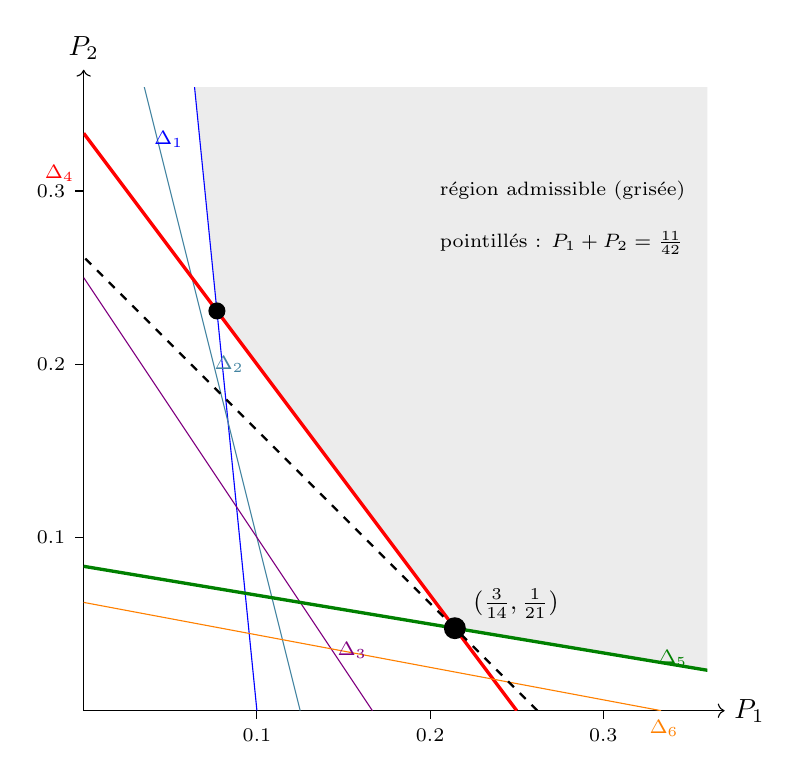
\begin{tikzpicture}[scale=22]
\draw[->] (0,0)--(0.37,0) node[right]{$P_1$};
\draw[->] (0,0)--(0,0.37) node[above]{$P_2$};
\foreach \t in {0.1,0.2,0.3} {\draw (\t,0)--(\t,-0.005) node[below]{\scriptsize\t}; \draw (0,\t)--(-0.005,\t) node[left]{\scriptsize\t};}
\begin{scope}
\clip (0,0) rectangle (0.36,0.36);
\fill[gray!15] (0,1)--(1/13,3/13)--(3/14,1/21)--(0.5,0)--(1,0)--(1,1)--cycle;
\draw[blue] (0.1,0)--(0.0,1.0);
\draw[cyan!60!black] (0.125,0)--(0,0.5);
\draw[violet] (1/6,0)--(0,0.25);
\draw[red,very thick] (0.25,0)--(0,1/3);
\draw[green!50!black,very thick] (0.5,0)--(0,1/12);
\draw[orange] (1/3,0)--(0,1/16);
\draw[dashed,thick] (11/42,0)--(0,11/42);
\end{scope}
\fill (3/14,1/21) circle (0.18pt); \fill (1/13,3/13) circle (0.14pt);
\node[above right] at (3/14+0.005,1/21) {\small $(\frac{3}{14},\frac{1}{21})$};
\node[blue,right] at (0.035,0.33) {\scriptsize $\Delta_1$};
\node[cyan!60!black,right] at (0.07,0.2) {\scriptsize $\Delta_2$};
\node[violet] at (0.155,0.035) {\scriptsize $\Delta_3$};
\node[red,left] at (0,0.31) {\scriptsize $\Delta_4$};
\node[green!50!black,above] at (0.34,0.02) {\scriptsize $\Delta_5$};
\node[orange,below] at (0.335,0) {\scriptsize $\Delta_6$};
\node[right] at (0.2,0.3) {\scriptsize région admissible (grisée)};
\node[right] at (0.2,0.27) {\scriptsize pointillés : $P_1+P_2=\frac{11}{42}$};
\end{tikzpicture}
\end{center}
La région admissible est l'intersection des demi-plans « au-dessus » des six droites. Pour chaque $P_1$, la contrainte la plus exigeante donne la frontière inférieure : successivement $\Delta_1$ (pour $0\le P_1\le\frac1{13}$), $\Delta_4$ (pour $\frac1{13}\le P_1\le\frac3{14}$), puis $\Delta_5$ (pour $\frac3{14}\le P_1\le\frac12$) ; $\Delta_2,\Delta_3,\Delta_6$ ne sont jamais actives. Les sommets sont
\[
(0,1),\quad \Big(\tfrac1{13},\tfrac3{13}\Big)=\Delta_1\cap\Delta_4,\quad \Big(\tfrac3{14},\tfrac1{21}\Big)=\Delta_4\cap\Delta_5,\quad \Big(\tfrac12,0\Big),
\]
où l'objectif vaut respectivement $1$, $\frac4{13}\approx0{,}308$, $\frac{11}{42}\approx0{,}262$, $\frac12$. Le minimum d'un programme linéaire étant atteint en un sommet, il est en $\Delta_4\cap\Delta_5$ :
\[\begin{cases}4P_1+3P_2=1\\ 2P_1+12P_2=1\end{cases}
\;\Rightarrow\; (4P_1+3P_2)-2(2P_1+12P_2)=1-2 \iff -21P_2=-1,
\]
\[
P_2=\tfrac1{21},\qquad P_1=\tfrac{1-3/21}{4}=\tfrac{3}{14}.
\]
\textbf{Contrôle des autres contraintes en ce point :}
\[
\Delta_1:\tfrac{30}{14}+\tfrac1{21}>1,\quad \Delta_2:\tfrac{24}{14}+\tfrac{2}{21}>1,\quad \Delta_3:\tfrac{18}{14}+\tfrac{4}{21}>1,\quad \Delta_6:\tfrac{9}{14}+\tfrac{16}{21}=\tfrac{59}{42}>1.
\]
Le point est admissible. \textbf{Optimalité :} pour un sommet sur $\Delta_4\cap\Delta_5$, l'objectif $(1,1)$ est combinaison positive des normales : $(1,1)=\lambda(4,3)+\mu(2,12)$ donne $\lambda=\frac{10}{42}=\frac5{21}>0$, $\mu=\frac1{42}>0$ ; le sommet est donc optimal (ces multiplicateurs sont précisément les $q_4,q_5$ du dual).
\[
P_1+P_2=\frac{3}{14}+\frac1{21}=\frac{9+2}{42}=\frac{11}{42}\;\Rightarrow\; v=\frac{42}{11},\quad x_1=P_1v=\frac{9}{11},\quad x_2=P_2v=\frac{2}{11}.
\]

\subsection*{Programme du joueur 2 (dual) et écarts complémentaires}
Avec $q_j=y_j/v$ :
\[
(II')\quad\begin{cases}
q_1+\dots+q_6\to\max\\
10q_1+8q_2+6q_3+4q_4+2q_5+3q_6\le1\\
q_1+2q_2+4q_3+3q_4+12q_5+16q_6\le1\\
q_j\ge0.
\end{cases}
\]
\textbf{Théorème des écarts complémentaires (T.E.C.)} :
\begin{itemize}
\item contraintes $\Delta_1,\Delta_2,\Delta_3,\Delta_6$ \emph{non saturées} (stricte) $\Rightarrow q_1=q_2=q_3=q_6=0$ ;
\item $P_1=\frac3{14}>0$ et $P_2=\frac1{21}>0\Rightarrow$ les deux contraintes de $(II')$ sont \emph{saturées} :
\end{itemize}
\[
\begin{cases}4q_4+2q_5=1\\3q_4+12q_5=1\end{cases}\;\Rightarrow\; q_4=\frac{12-2}{48-6}=\frac{10}{42}=\frac5{21},\quad q_5=\frac{4-3}{42}=\frac1{42}.
\]
Contrôle : $q_4+q_5=\frac{11}{42}=P_1+P_2$ (égalité des valeurs optimales primal/dual). Alors $y_4=q_4v=\frac{10}{11}$, $y_5=q_5v=\frac1{11}$.
\[
\boxed{x^*=\Big(\frac{9}{11},\frac{2}{11}\Big),\qquad y^*=\Big(0,0,0,\frac{10}{11},\frac{1}{11},0\Big),\qquad v=\frac{42}{11}\approx3{,}818.}
\]
\textbf{Vérification (Théorème 2).}
$x^{*T}A=\frac1{11}(92,\,76,\,62,\,42,\,42,\,59)\ge\frac{42}{11}$ et $Ay^*=\frac1{11}(42,\,42)^T\le\frac{42}{11}$. \checkmark

\begin{rembox}{Contrôle par la méthode graphique (joueur 1)}
Avec $x=(p,1-p)$ : $C_1:1+9p$, $C_2:2+6p$, $C_3:4+2p$, $C_4:3+p$, $C_5:12-10p$, $C_6:16-13p$. L'enveloppe inférieure est $\min(1+9p,\,3+p)$ côté croissant et $12-10p$ côté décroissant ; le maximum est $3+p=12-10p\iff p=\frac9{11}$, $v=\frac{42}{11}$. Même résultat.
\end{rembox}

%=====================================================================
\section*{Exercice 5 : Propriétés des solutions optimales}

Soit $(x,y)$ une solution et $v$ la valeur. D'après le Théorème 2 :
\[
(\ast)\;\sum_{i=1}^m a_{ij}x_i\ge v\ \ (j=1..n),\qquad (\ast\ast)\;\sum_{j=1}^n a_{ij}y_j\le v\ \ (i=1..m),\qquad x,y\ge0,\ \sum x_i=\sum y_j=1.
\]
\textbf{Lemme : $E(x,y)=v$.} En multipliant $(\ast)$ par $y_j\ge0$ et en sommant : $E(x,y)=\sum_j y_j\sum_i a_{ij}x_i\ge v\sum_j y_j=v$. De même avec $(\ast\ast)$ et $x_i$ : $E(x,y)\le v$. Donc $E(x,y)=v$.

\subsection*{1. Si $\sum_j a_{i_0j}y_j<v$ alors $x_{i_0}=0$}
Notons $g_i=\sum_j a_{ij}y_j$ (gain du joueur 1 s'il joue la ligne pure $i$ contre $y$). Par $(\ast\ast)$, $v-g_i\ge0$ pour tout $i$, et par le lemme
\[
\sum_{i=1}^m x_i\,(v-g_i)=v\sum_i x_i-\sum_i x_ig_i=v-E(x,y)=0.
\]
C'est une somme de termes \emph{positifs ou nuls} ($x_i\ge0$, $v-g_i\ge0$) de somme nulle : chaque terme est nul, $x_i(v-g_i)=0$ pour tout $i$. Pour $i=i_0$, $v-g_{i_0}>0$, donc
\[
\boxed{x_{i_0}=0.}
\]
\emph{Interprétation :} une ligne qui rapporte strictement moins que $v$ contre la stratégie optimale de l'adversaire n'est jamais jouée.

\subsection*{2. Si $\sum_i a_{ij_0}x_i>v$ alors $y_{j_0}=0$}
\begin{rembox}{Remarque sur l'énoncé}
L'énoncé écrit « $\sum_i a_{ij_0}x_i<v$ », ce qui est impossible d'après $(\ast)$ (la proposition serait vraie mais vide). La propriété symétrique utile, celle employée dans le cours (p.~29--30, relation $(\ast\ast)$ : $4\cdot\frac23>v\Rightarrow y_3=0$), est avec $>$. On démontre celle-ci.
\end{rembox}
Notons $h_j=\sum_i a_{ij}x_i$. Par $(\ast)$, $h_j-v\ge0$, et
\[
\sum_{j=1}^n y_j\,(h_j-v)=E(x,y)-v=0.
\]
Somme de termes positifs ou nuls de somme nulle : $y_j(h_j-v)=0$ pour tout $j$. Pour $j_0$, $h_{j_0}-v>0$, d'où
\[
\boxed{y_{j_0}=0.}
\]
\emph{Interprétation :} une colonne qui coûte au joueur 2 strictement plus que $v$ face à $x$ optimal n'est jamais jouée. Ce sont exactement les relations du \textbf{théorème des écarts complémentaires} appliquées aux programmes $(I')$ et $(II')$.

\vspace{0.5cm}
\begin{verifbox}
Toutes les valeurs ci-dessus ont été recontrôlées en arithmétique exacte (\texttt{fractions}) et par programmation linéaire (\texttt{scipy.optimize.linprog}) dans \texttt{verification\_TDJ.py} : point selle $(2,1)$ de l'Ex.~1 ; $v=\frac{10}{3}$ de l'Ex.~2 ; convexité/concavité de l'Ex.~3 ; $P=(\frac3{14},\frac1{21})$, contraintes saturées $\Delta_4,\Delta_5$ seulement, $q_4=\frac5{21}$, $q_5=\frac1{42}$ et $v=\frac{42}{11}$ de l'Ex.~4.
\end{verifbox}

\end{document}
